\documentclass{standalone}
\usepackage{tikz}
\usetikzlibrary{patterns, positioning}
\usepackage[sfdefault]{ClearSans} %% option 'sfdefault' activates Clear Sans as the default text font
\usepackage[T1]{fontenc}

\begin{document}
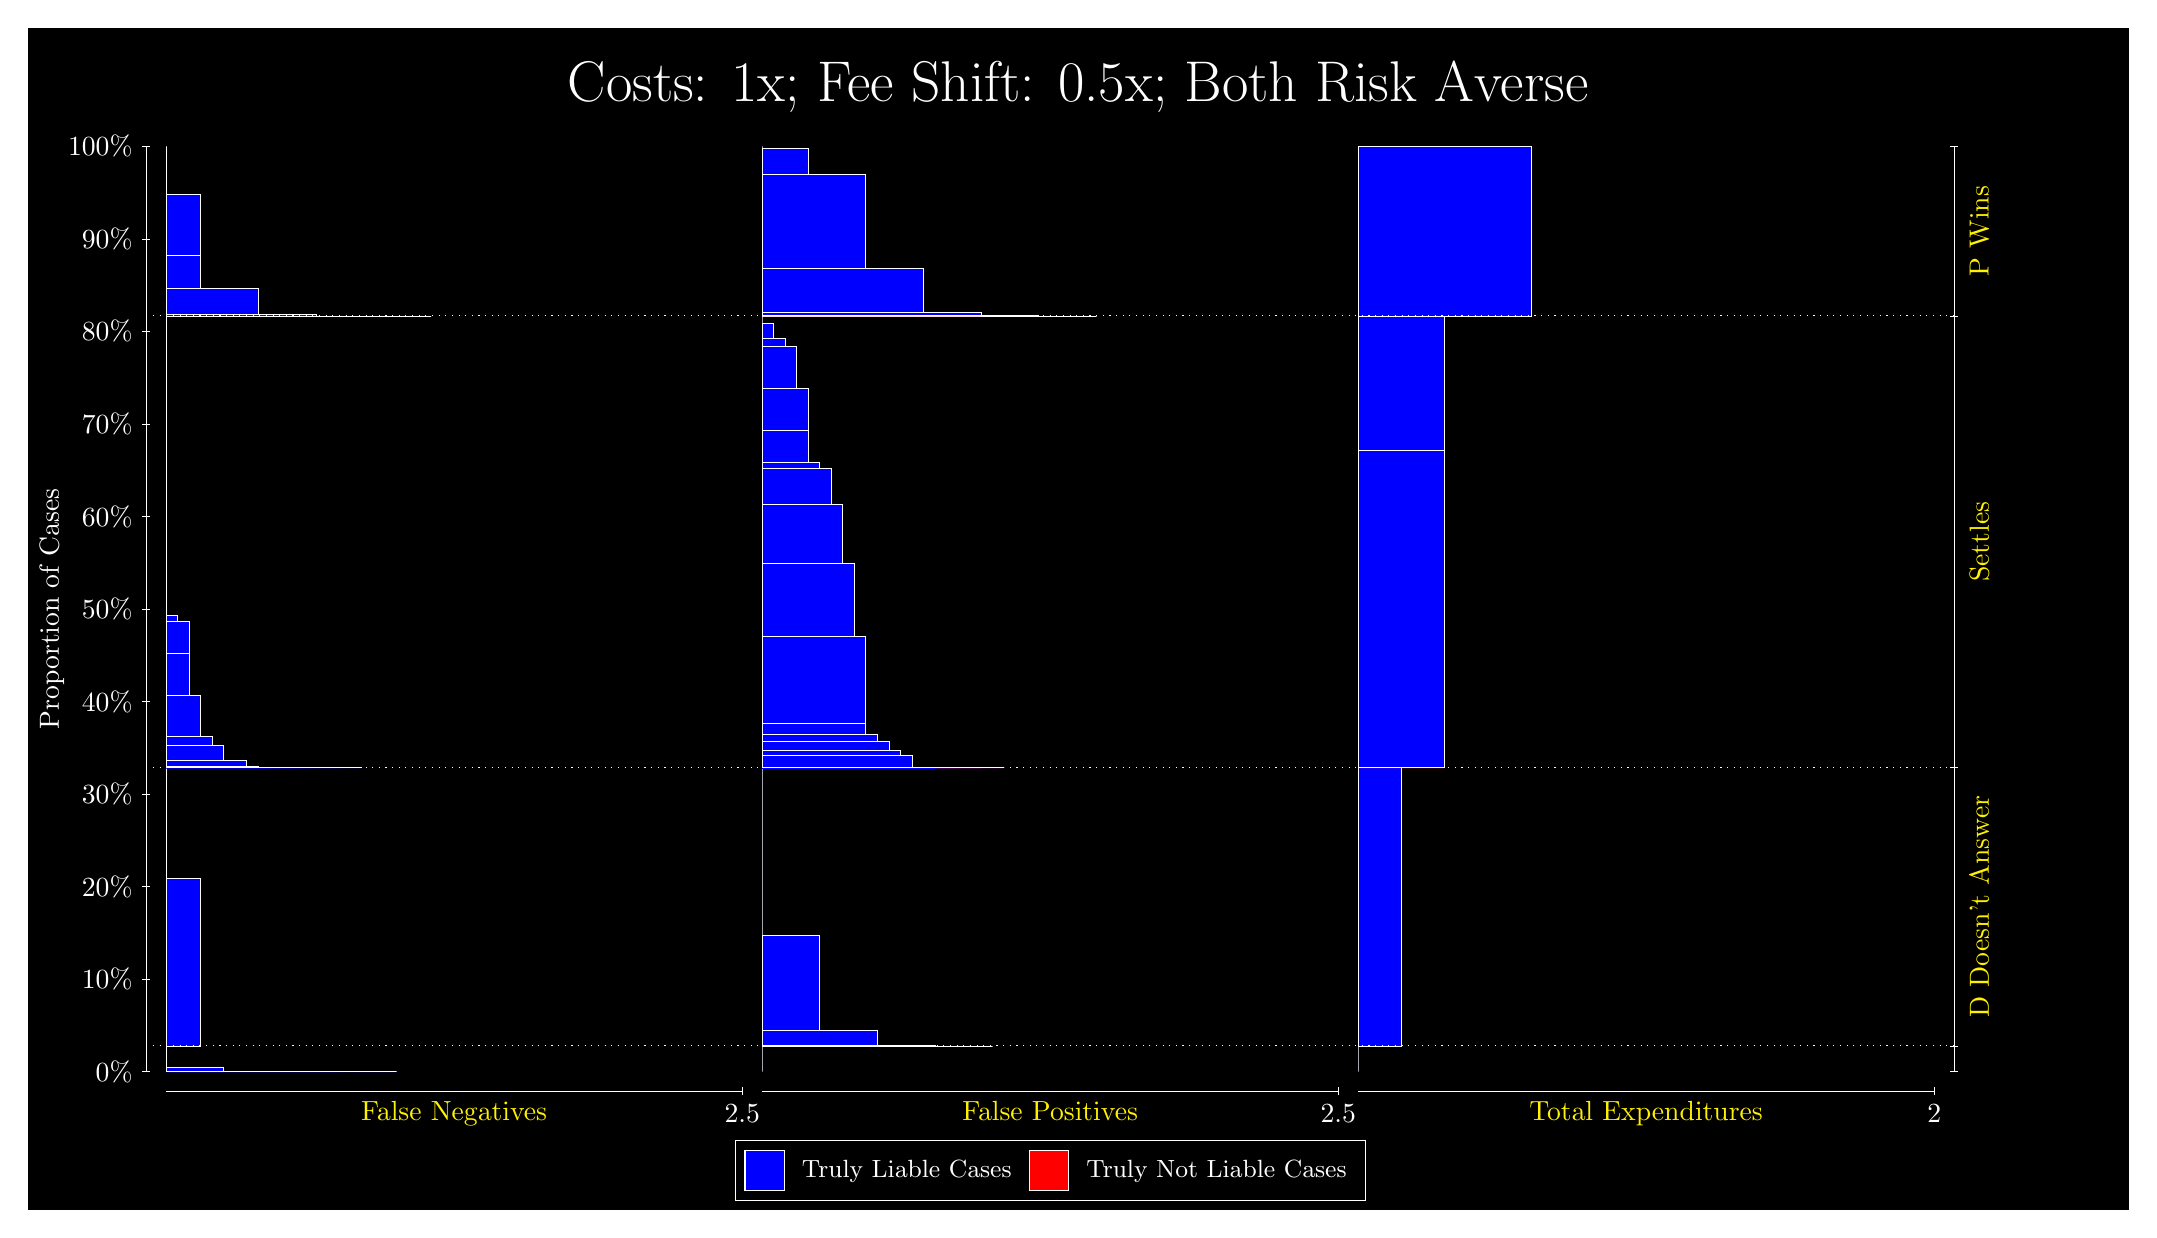
\begin{tikzpicture}
\draw[fill=black] (0,0) rectangle (26.667,15);
\draw[text=white] (0,13.5) rectangle (26.667,15) node[midway] {\huge Costs: 1x; Fee Shift: 0.5x; Both Risk Averse};
\draw[white, very thin] (1.5,1.75) -- (1.5,13.5);
\node[rotate=90, text=white, anchor=center] at (0.3, 7.625) {Proportion of Cases};
\draw[white, very thin] (1.45,1.75) -- (1.55,1.75);
\node[text=white, anchor=east] at (1.45, 1.75) {0\%};
\draw[white, very thin] (1.45,2.925) -- (1.55,2.925);
\node[text=white, anchor=east] at (1.45, 2.925) {10\%};
\draw[white, very thin] (1.45,4.1) -- (1.55,4.1);
\node[text=white, anchor=east] at (1.45, 4.1) {20\%};
\draw[white, very thin] (1.45,5.275) -- (1.55,5.275);
\node[text=white, anchor=east] at (1.45, 5.275) {30\%};
\draw[white, very thin] (1.45,6.45) -- (1.55,6.45);
\node[text=white, anchor=east] at (1.45, 6.45) {40\%};
\draw[white, very thin] (1.45,7.625) -- (1.55,7.625);
\node[text=white, anchor=east] at (1.45, 7.625) {50\%};
\draw[white, very thin] (1.45,8.8) -- (1.55,8.8);
\node[text=white, anchor=east] at (1.45, 8.8) {60\%};
\draw[white, very thin] (1.45,9.975) -- (1.55,9.975);
\node[text=white, anchor=east] at (1.45, 9.975) {70\%};
\draw[white, very thin] (1.45,11.15) -- (1.55,11.15);
\node[text=white, anchor=east] at (1.45, 11.15) {80\%};
\draw[white, very thin] (1.45,12.325) -- (1.55,12.325);
\node[text=white, anchor=east] at (1.45, 12.325) {90\%};
\draw[white, very thin] (1.45,13.5) -- (1.55,13.5);
\node[text=white, anchor=east] at (1.45, 13.5) {100\%};

\draw[white, very thin] (24.457,1.75) -- (24.457,13.5);
\draw[white, very thin] (24.407,1.75) -- (24.507,1.75);
\node[anchor=west] at (24.407, 1.75) {};
\draw[white, very thin] (24.407,2.0757) -- (24.507,2.0757);
\node[anchor=west] at (24.407, 2.0757) {};
\draw[white, very thin] (24.407,5.61) -- (24.507,5.61);
\node[anchor=west] at (24.407, 5.61) {};
\draw[white, very thin] (24.407,11.347) -- (24.507,11.347);
\node[anchor=west] at (24.407, 11.347) {};
\draw[white, very thin] (24.407,13.5) -- (24.507,13.5);
\node[anchor=west] at (24.407, 13.5) {};

\draw[white, very thin, fill=blue] (1.75,1.75) rectangle (4.6775,1.75);
\draw[white, very thin, fill=blue] (1.75,1.75) rectangle (3.9457,1.75);
\draw[white, very thin, fill=blue] (1.75,1.75) rectangle (3.2138,1.7505);
\draw[white, very thin, fill=blue] (1.75,1.7505) rectangle (2.4819,1.8033);
\draw[white, very thin, fill=red] (1.75,1.8033) rectangle (1.75,1.8033);
\draw[white, very thin, fill=blue] (1.75,1.8033) rectangle (1.75,2.0757);
\draw[white, very thin, fill=blue] (1.75,2.0757) rectangle (2.1891,4.2103);
\draw[white, very thin, fill=red] (1.75,4.2103) rectangle (1.75,4.2103);
\draw[white, very thin, fill=blue] (1.75,4.2103) rectangle (1.75,5.61);
\draw[white, very thin, fill=blue] (1.75,5.61) rectangle (4.2384,5.61);
\draw[white, very thin, fill=blue] (1.75,5.61) rectangle (3.9457,5.61);
\draw[white, very thin, fill=blue] (1.75,5.61) rectangle (3.6529,5.61);
\draw[white, very thin, fill=blue] (1.75,5.61) rectangle (3.5065,5.61);
\draw[white, very thin, fill=blue] (1.75,5.61) rectangle (3.3602,5.61);
\draw[white, very thin, fill=blue] (1.75,5.61) rectangle (3.2138,5.61);
\draw[white, very thin, fill=blue] (1.75,5.61) rectangle (3.0674,5.6102);
\draw[white, very thin, fill=blue] (1.75,5.6102) rectangle (2.921,5.6273);
\draw[white, very thin, fill=blue] (1.75,5.6273) rectangle (2.7746,5.7016);
\draw[white, very thin, fill=blue] (1.75,5.7016) rectangle (2.6283,5.702);
\draw[white, very thin, fill=blue] (1.75,5.702) rectangle (2.4819,5.8929);
\draw[white, very thin, fill=blue] (1.75,5.8929) rectangle (2.3355,6.0027);
\draw[white, very thin, fill=blue] (1.75,6.0027) rectangle (2.1891,6.5302);
\draw[white, very thin, fill=blue] (1.75,6.5302) rectangle (2.0428,7.0664);
\draw[white, very thin, fill=blue] (1.75,7.0664) rectangle (2.0428,7.466);
\draw[white, very thin, fill=blue] (1.75,7.466) rectangle (1.8964,7.5456);
\draw[white, very thin, fill=red] (1.75,7.5456) rectangle (1.75,7.5456);
\draw[white, very thin, fill=blue] (1.75,7.5456) rectangle (1.75,11.347);
\draw[white, very thin, fill=blue] (1.75,11.347) rectangle (5.1167,11.347);
\draw[white, very thin, fill=blue] (1.75,11.347) rectangle (4.3848,11.347);
\draw[white, very thin, fill=blue] (1.75,11.347) rectangle (3.6529,11.366);
\draw[white, very thin, fill=blue] (1.75,11.366) rectangle (2.921,11.702);
\draw[white, very thin, fill=blue] (1.75,11.702) rectangle (2.1891,12.12);
\draw[white, very thin, fill=blue] (1.75,12.12) rectangle (2.1891,12.897);
\draw[white, very thin, fill=red] (1.75,12.897) rectangle (1.75,12.897);
\draw[white, very thin, fill=blue] (1.75,12.897) rectangle (1.75,13.5);
\draw[white, very thin, fill=red] (9.3189,1.75) rectangle (9.3189,1.75);
\draw[white, very thin, fill=blue] (9.3189,1.75) rectangle (9.3189,2.0757);
\draw[white, very thin, fill=red] (9.3189,2.0757) rectangle (12.246,2.0757);
\draw[white, very thin, fill=blue] (9.3189,2.0757) rectangle (12.246,2.0757);
\draw[white, very thin, fill=blue] (9.3189,2.0757) rectangle (11.515,2.0774);
\draw[white, very thin, fill=blue] (9.3189,2.0774) rectangle (10.783,2.2722);
\draw[white, very thin, fill=blue] (9.3189,2.2722) rectangle (10.051,3.4754);
\draw[white, very thin, fill=blue] (9.3189,3.4754) rectangle (9.3189,5.61);
\draw[white, very thin, fill=red] (9.3189,5.61) rectangle (12.393,5.61);
\draw[white, very thin, fill=blue] (9.3189,5.61) rectangle (12.393,5.61);
\draw[white, very thin, fill=red] (9.3189,5.61) rectangle (12.1,5.61);
\draw[white, very thin, fill=blue] (9.3189,5.61) rectangle (12.1,5.61);
\draw[white, very thin, fill=red] (9.3189,5.61) rectangle (11.807,5.61);
\draw[white, very thin, fill=blue] (9.3189,5.61) rectangle (11.807,5.6101);
\draw[white, very thin, fill=blue] (9.3189,5.6101) rectangle (11.661,5.6101);
\draw[white, very thin, fill=red] (9.3189,5.6101) rectangle (11.515,5.6101);
\draw[white, very thin, fill=blue] (9.3189,5.6101) rectangle (11.515,5.6107);
\draw[white, very thin, fill=blue] (9.3189,5.6107) rectangle (11.368,5.6112);
\draw[white, very thin, fill=red] (9.3189,5.6112) rectangle (11.222,5.6112);
\draw[white, very thin, fill=blue] (9.3189,5.6112) rectangle (11.222,5.7618);
\draw[white, very thin, fill=blue] (9.3189,5.7618) rectangle (11.075,5.832);
\draw[white, very thin, fill=red] (9.3189,5.832) rectangle (10.929,5.832);
\draw[white, very thin, fill=blue] (9.3189,5.832) rectangle (10.929,5.9479);
\draw[white, very thin, fill=blue] (9.3189,5.9479) rectangle (10.783,6.0289);
\draw[white, very thin, fill=blue] (9.3189,6.0289) rectangle (10.636,6.1721);
\draw[white, very thin, fill=red] (9.3189,6.1721) rectangle (10.636,6.1721);
\draw[white, very thin, fill=blue] (9.3189,6.1721) rectangle (10.636,7.284);
\draw[white, very thin, fill=blue] (9.3189,7.284) rectangle (10.49,8.2062);
\draw[white, very thin, fill=blue] (9.3189,8.2062) rectangle (10.344,8.9579);
\draw[white, very thin, fill=blue] (9.3189,8.9579) rectangle (10.197,9.4117);
\draw[white, very thin, fill=blue] (9.3189,9.4117) rectangle (10.051,9.4912);
\draw[white, very thin, fill=blue] (9.3189,9.4912) rectangle (9.9044,9.8908);
\draw[white, very thin, fill=blue] (9.3189,9.8908) rectangle (9.9044,10.427);
\draw[white, very thin, fill=blue] (9.3189,10.427) rectangle (9.758,10.955);
\draw[white, very thin, fill=blue] (9.3189,10.955) rectangle (9.6116,11.064);
\draw[white, very thin, fill=blue] (9.3189,11.064) rectangle (9.4652,11.255);
\draw[white, very thin, fill=blue] (9.3189,11.255) rectangle (9.3189,11.347);
\draw[white, very thin, fill=red] (9.3189,11.347) rectangle (13.564,11.347);
\draw[white, very thin, fill=blue] (9.3189,11.347) rectangle (13.564,11.347);
\draw[white, very thin, fill=red] (9.3189,11.347) rectangle (12.832,11.347);
\draw[white, very thin, fill=blue] (9.3189,11.347) rectangle (12.832,11.348);
\draw[white, very thin, fill=red] (9.3189,11.348) rectangle (12.1,11.348);
\draw[white, very thin, fill=blue] (9.3189,11.348) rectangle (12.1,11.396);
\draw[white, very thin, fill=red] (9.3189,11.396) rectangle (11.368,11.396);
\draw[white, very thin, fill=blue] (9.3189,11.396) rectangle (11.368,11.95);
\draw[white, very thin, fill=red] (9.3189,11.95) rectangle (10.636,11.95);
\draw[white, very thin, fill=blue] (9.3189,11.95) rectangle (10.636,13.145);
\draw[white, very thin, fill=blue] (9.3189,13.145) rectangle (9.9044,13.481);
\draw[white, very thin, fill=blue] (9.3189,13.481) rectangle (9.3189,13.5);
\draw[white, very thin, fill=red] (16.888,1.75) rectangle (16.888,1.75);
\draw[white, very thin, fill=blue] (16.888,1.75) rectangle (16.888,2.0757);
\draw[white, very thin, fill=red] (16.888,2.0757) rectangle (17.437,2.0757);
\draw[white, very thin, fill=blue] (16.888,2.0757) rectangle (17.437,5.61);
\draw[white, very thin, fill=red] (16.888,5.61) rectangle (17.986,5.61);
\draw[white, very thin, fill=blue] (16.888,5.61) rectangle (17.986,9.6459);
\draw[white, very thin, fill=red] (16.888,9.6459) rectangle (17.986,9.6459);
\draw[white, very thin, fill=blue] (16.888,9.6459) rectangle (17.986,11.347);
\draw[white, very thin, fill=red] (16.888,11.347) rectangle (19.083,11.347);
\draw[white, very thin, fill=blue] (16.888,11.347) rectangle (19.083,13.5);
\draw[white, dotted] (1.5,2.0757) -- (24.457,2.0757);
\draw[white, dotted] (1.5,5.61) -- (24.457,5.61);
\draw[white, dotted] (1.5,11.347) -- (24.457,11.347);
\draw[white, very thin] (1.75,1.5) -- (9.0689,1.5);
\node[text=yellow, anchor=north] at (5.4094, 1.5) {False Negatives};
\draw[white, very thin] (9.0689,1.45) -- (9.0689,1.55);
\node[text=white, anchor=north] at (9.0689, 1.45) {2.5};

\draw[white, very thin] (9.3189,1.5) -- (16.638,1.5);
\node[text=yellow, anchor=north] at (12.978, 1.5) {False Positives};
\draw[white, very thin] (16.638,1.45) -- (16.638,1.55);
\node[text=white, anchor=north] at (16.638, 1.45) {2.5};

\draw[white, very thin] (16.888,1.5) -- (24.207,1.5);
\node[text=yellow, anchor=north] at (20.547, 1.5) {Total Expenditures};
\draw[white, very thin] (24.207,1.45) -- (24.207,1.55);
\node[text=white, anchor=north] at (24.207, 1.45) {2};


\node[text=yellow, centered, rotate=90] at (24.777, 3.8428) {D Doesn't Answer};
\node[text=yellow, centered, rotate=90] at (24.777, 8.4786) {Settles};
\node[text=yellow, centered, rotate=90] at (24.777, 12.424) {P Wins};

\draw (12.978300999999998,1.5) node[draw=none] (baseCoordinate) {};
\begin{scope}[align=center]
        \matrix[scale=0.5, draw=white, below=0.5cm of baseCoordinate, nodes={draw}, column sep=0.1cm]{
            \node[rectangle, draw, minimum width=0.5cm, minimum height=0.5cm, fill=blue] {}; &
            \node[draw=none, font=\small, text=white] (B) {Truly Liable Cases}; &
            \node[rectangle, draw, minimum width=0.5cm, minimum height=0.5cm, fill=red] {}; &
            \node[draw=none, font=\small, text=white] (B) {Truly Not Liable Cases}; \\
            };
\end{scope}

\end{tikzpicture}
\end{document}